\section{Old}

\subsection{Computing Posterior Distribution by Initially Applying Bayes Rule}

  There is another way we can approach to calculating the posterior $p(\theta\,|\,\mathcal{D})$.

  \begin{enumerate}
    \item We directly apply Bayes rule to get
    \begin{equation}
      p(\theta\,|\,\mathcal{D}) = \frac{p(\mathcal{D}\,|\,\theta)\, p(\theta)}{p(\mathcal{D})} = \frac{p(\mathcal{D}\,|\,\theta)\, p(\theta)}{\int p(\mathcal{D}\,|\,\theta)\, p(\theta)\; d\theta}
    \end{equation}
    Since we are working under a specific model $\mathcal{M}_i$, it would be more accurate to say
    \begin{equation}
      p(\theta^i \,|\,\mathcal{D}, \mathcal{M}_i) = \frac{p(\mathcal{D}\,|\,\theta^i, \mathcal{M}_i)\, p(\theta^i \,|\,\mathcal{M}_i)}{p(\mathcal{D}\,|\,\mathcal{M}_i)} = \frac{p(\mathcal{D}\,|\,\theta^i, \mathcal{M}_i)\, p(\theta^i \,|\,\mathcal{M}_i)}{\int p(\mathcal{D}\,|\,\theta^i, \mathcal{M}_i)\, p(\theta^i \,|\,\mathcal{M}_i)\; d\theta^i}
    \end{equation}

    \item Since $\mathcal{D} = \{(x_i, y_i)\}_{i=1}^N$ consists of $N$ independent observations, we can calculate
    \begin{equation}
      p(\mathcal{D}\,|\,\theta^i , \mathcal{M}_i) = \prod_{j=1}^N p(y_j \,|\,x_j, \theta^i, \mathcal{M}_i)
    \end{equation}
    since the form of the likelihood is determined by our model $\mathcal{M}_i$ that says $y = f(x, \theta^i) + \epsilon$.

    \item To calculate $p(\theta^i\,|\,\mathcal{M}_i)$, we would have to condition over the hyperparameter $\gamma$, which gives
    \begin{equation}
      p(\theta^i \,|\,\mathcal{M}_i) = \int p(\theta^i\,|\,\gamma, \mathcal{M}_i)\, p(\gamma\,|\,\mathcal{M}_i)\; d\gamma
    \end{equation}
    where $p(\theta^i\,|\,\gamma, \mathcal{M}_i)$ is the density of $\text{Dist}_{\theta^i} (\gamma)$ where $\gamma$ is constant, and $p(\gamma\,|\,\mathcal{M}_i)$ is the prior distribution $\text{Dist}_\gamma (\xi)$ with fixed $\xi$.
  \end{enumerate}

  Multiplying the two would get the proportional term, and integrating them over $\theta^i$ would get the marginalization constant
  \begin{equation}
    p(\mathcal{D}\,|\,\mathcal{M}_i) = \int p(\mathcal{D}\,|\,\theta^i, \mathcal{M}_i) \, p(\theta^i\,|\,\mathcal{M}_i)\; d\theta^i
  \end{equation}
  entirely defining the posterior. Upon closer inspection, these two methods of deriving the posterior parameter are not that different. One just uses Bayes rule first and then marginalizes, while the other marginalizes and then uses Bayes rule.

\subsection{Constructing a Predictive Function from Parameter Density}

  We can then construct a \textbf{predictive distribution} that calculates the probability of $y$ given $x$. That is, given a new input $x$, the probability of getting a value $y$, given our dataset $\mathcal{D}$, is
  \begin{align*}
    p(y\,|\,x, \mathcal{D}, \mathcal{M}_i) & = \int p(y\,|\,\theta^i, x, \mathcal{D}, \mathcal{M}_i) \, p(\theta^i \,|\, x, \mathcal{D}, \mathcal{M}_i)\; d\theta^i \\
    & = \int p(y\,|\,\theta^i, x, \mathcal{M}_i)\, p(\theta^i \,|\,\mathcal{D}, \mathcal{M}_i)\; d\theta^i
  \end{align*}
  but $p(\theta^i\,|\,\mathcal{D}, \mathcal{M}_i)$ is completely defined by what we just calculated, and $p(y\,|\,\theta^i, x, \mathcal{D}, \mathcal{M}_i)$ is defined by the random variable generated by
  \begin{equation}
    y \sim f(x, \theta^i) + \epsilon
  \end{equation}

\subsection{Bayesian Model Selection}

  Note that up until now, we have assumed that we \textit{knew} the \textbf{statistical model} describing the process of how the data $\mathcal{D}$ was generated. The definition of a model is often used loosely without explicit definition, but we can define it as such: A model completely defines the \textit{form} of the function $f$ that we assume is generating $y$ for values of $x$. This does not mean that the model corresponds to a parameter value of $w$. It defines the \textit{entire form} of $f$ for
  \begin{equation}
    y = f(x, \theta) + \epsilon
  \end{equation}

  The model then defines the form of $p(y_i\,|\,x_i, \theta)$ according to the above, which then defines the form of the likelihood function
  \begin{equation}
    p(\mathcal{D}\,|\,\theta) = \prod_{i=1}^N p(y_i\,|\,x_i, \theta)
  \end{equation}

  Here are some examples of different models for different problems. Note that for every model $\mathcal{M}_i$, the set of parameters $\theta^i$ is \textit{different}, since the basis functions do not need to necessarily be the same for these models.

  \begin{enumerate}
    \item For linear regression, we assume that the distribution is of form
    \begin{equation}
      y = w^T \phi(x) + \epsilon
    \end{equation}
    and thus our models have different forms which are completely dependent on the basis functions $\phi_j(x)$ we choose. Assuming that we have scalar inputs $x \in \mathbb{R}$, we may choose
    \begin{itemize}
      \item a purely linear model of $x$, which we will call $\mathcal{M}_1$ with $\theta^1 = (w_0, w_1)$.
      \begin{equation}
        y = \begin{pmatrix} w_0 & w_1 \end{pmatrix} \begin{pmatrix} \phi_0 (x) \\ \phi_1 (x) \end{pmatrix} + \epsilon = \begin{pmatrix} w_0 & w_1 \end{pmatrix} \begin{pmatrix} 1 \\ x \end{pmatrix} + \epsilon
      \end{equation}
      Therefore the form is $f(x, w) = w_0 + w_1 x$.

      \item a quadratic model of $x$, which we will call $\mathcal{M}_2$ with $\theta^2 = (w_0, w_1, w_2)$.
      \begin{equation}
        y = \begin{pmatrix} w_0 & w_1 & w_2 \end{pmatrix} \begin{pmatrix} \phi_0 (x) \\ \phi_1 (x) \\ \phi_2 (x) \end{pmatrix} + \epsilon = \begin{pmatrix} w_0 & w_1 & w_2 \end{pmatrix} \begin{pmatrix} 1 \\ x \\ x^2 \end{pmatrix} + \epsilon
      \end{equation}
      Therefore the form is $f(x, w) = w_0 + w_1 x + w_2 x^2$.

      \item a cubic model of $x$ called $\mathcal{M}_3$ with form $f(x, \theta) = w_0 + w_1 x + w_2 x^2 + w_3 x^3$, and so on...
    \end{itemize}
    \item More examples to be updated.
  \end{enumerate}

  A fully Bayesian approach would condition over all possible models when predicting $y$ given $x$. Suppose that we have a finite set of Bayesian models $\{\mathcal{M}_i\}$ (each with their own parameters $\theta^i$) that we could use to explain the observed data $\mathcal{D}$. Then, as shown above, for each $i$th model, we would calculate the posterior density of the parameter $p(\theta^i\,|\,\mathcal{D}, \mathcal{M}_i)$ and then construct a predictive distribution
  \begin{equation}
    p(y\,|\,x, \mathcal{D}, \mathcal{M}_i)
  \end{equation}

  for each model in $\{\mathcal{M}_i\}$. Then we calculate the posterior probabilities of the models $p(\mathcal{M}_i\,|\,\mathcal{D})$, and conditioning over all possible models, we get the ultimate predictive distribution over all models
  \begin{equation}
    p(y\,|\,x, \mathcal{D}) = \sum_i p(y\,|\,x, \mathcal{D}, \mathcal{M}_i)\, p(\mathcal{M}_i\,|\,\mathcal{D})
  \end{equation}

  This is called a \textbf{mixture model} or \textbf{Bayesian model averaging}, but in practice this is not used due to computational overhead. A more common practice is simply to calculate all the $p(\mathcal{M}_i\,|\,\mathcal{D})$, pick the $\mathcal{M}_i$ that has the highest posterior probability, and build out predictive distribution assuming $\mathcal{M}_i$. This is called \textbf{model selection}, since we are throwing away all other models that are deemed to overfit or underfit and selecting the best one.

  Now, the problem of model selection (and averaging) reduces to just finding the posterior model probabilities $p(\mathcal{M}_i \,|\,\mathcal{D})$, since we know how to do everything else. We can work out the posterior probability over the models via Bayes rule
  \begin{equation}
    p(\mathcal{M}_i \,|\,\mathcal{D}) \propto p(\mathcal{D}\,|\,\mathcal{M}_i)\, p(\mathcal{M}_i)
  \end{equation}

  $p(\mathcal{M}_i)$ is the prior distribution over models that we have selected, which is conventionally set to the uniform: $p(\mathcal{M}_i) \propto 1$. Therefore, calculating the posterior probability of the models reduces to calculating $p(\mathcal{D}\,|\,\mathcal{M}_i)$ which is called the \textbf{model evidence}. By marginalizing over the parameter $\theta^i$, we have
  \begin{equation}
    p(\mathcal{D}\,|\,\mathcal{M}_i) = \int p(\mathcal{D}\,|\,\theta^i, \mathcal{M}_i) \, p(\theta^i\,|\,\mathcal{M}_i)\; d\theta^i
  \end{equation}

  To calculate this, we evaluate each component of the integral:
  \begin{itemize}
    \item Remember that $\mathcal{D} = \{(x_i, y_i)\}_{i=1}^N$ is composed of independent data. So
    \begin{equation}
      p(\mathcal{D}\,|\,\theta^i, \mathcal{M}_i) = \prod_{i=1}^N p(y_i \,|\, x_i, \theta^i, \mathcal{M}_i)
    \end{equation}
    which is well-defined since we can simply use our model $y = f (x, \theta^i) + \epsilon$.

    \item Furthermore, we see that $p(\theta^i \,|\,\mathcal{M}_i)$ should be conditioned over its hyperparameter $\gamma$, so
    \begin{equation}
      p(\theta^i \,|\,\mathcal{M}_i) = \int p(\theta^i \,|\,\gamma, \mathcal{M}_i) \, p(\gamma\,|\,\mathcal{M}_i)\; d\gamma
    \end{equation}
    where $\theta^i \,|\,\gamma \sim \text{Dist}_\theta (\gamma)$ for constant $\gamma$ and $\gamma \sim \text{Dist}_\gamma (\xi)$ for constant $\xi$.
  \end{itemize}

  Note that if we had calculated the posterior densities of the parameters $p(\theta_i\,|\,\mathcal{D}, \mathcal{M}_i)$ by applying Bayes rule first, we would have calculated the posterior as
  \begin{equation}
    p(\theta^i\,|\,\mathcal{D}, \mathcal{M}_i) = \frac{p(\mathcal{D}\,|\,\theta^i, \mathcal{M}_i)\, p(\theta^i \,|\,\mathcal{M}_i)}{p(\mathcal{D}\,|\,\mathcal{M}_i)} = \frac{p(\mathcal{D}\,|\,\theta^i, \mathcal{M}_i)\, p(\theta^i \,|\,\mathcal{M}_i)}{\int p(\mathcal{D}\,|\,\theta^i, \mathcal{M}_i)\, p(\theta^i \,|\,\mathcal{M}_i)\; d\theta^i}
  \end{equation}

  Note that the marginalization term that we've already calculated is the model evidence! So this shortcut may save us a lot of computation.

\subsection{Intuition Behind Model Evidence}

  Let us take a closer look at the model evidence term and try to develop an intuition for it.
  \begin{equation}
    p(\mathbf{Y} \,|\,\mathcal{M}_i) = \int p(\mathbf{Y}\,|\,w, \mathcal{M}_i) p(w\,|\,\mathcal{M}_i) \; dw
  \end{equation}

  Note that the evidence tells us the probability of getting $\mathbf{Y}$ from a given model $\mathcal{M}_i$, and we want this to be as large as possible. It does this by conditioning over all possible values of $w$ for that given model. Consider first the case of a model having a single parameter $w$. Let us make two assumptions:
  \begin{itemize}
    \item The posterior distribution $p(\mathbf{Y}\,|\,w, \mathcal{M}_i)$ is sharply peaked around the most probable value $w_{MAP}$, with width $\Delta w_{\text{posterior}}$.
    \item The prior distribution $p(w\,|,\mathcal{M}_i)$ is flat with width $\Delta w_{\text{prior}}$, so that $p(w) = 1/ \Delta w_{\text{prior}}$.
  \end{itemize}

  \begin{figure}[H]
    \centering
    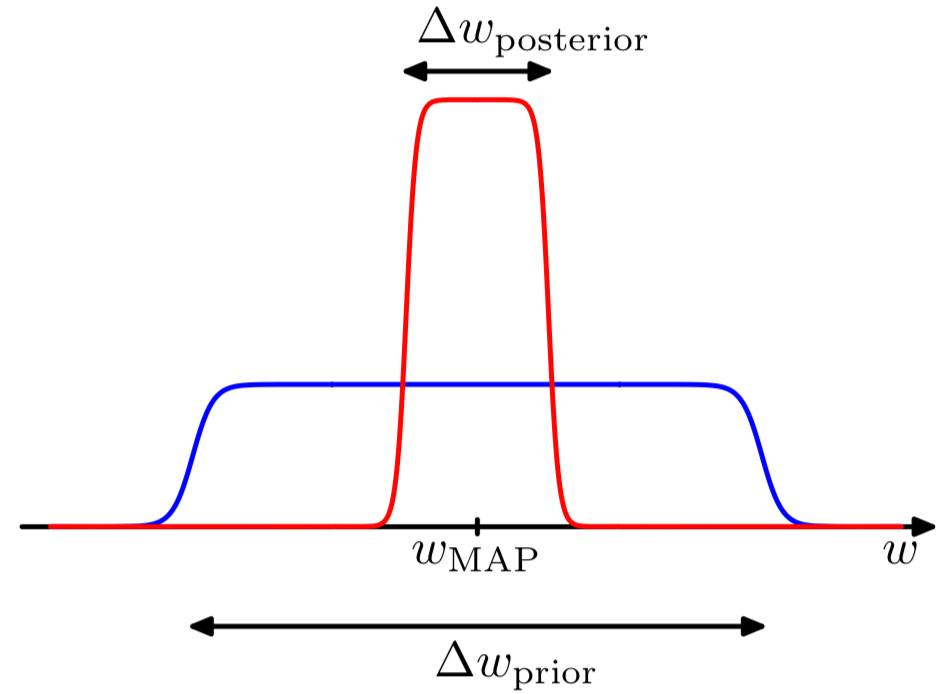
\includegraphics[width=0.4\textwidth]{img/approximation.jpg}
    \caption{Approximation of posterior and prior distributions}
  \end{figure}

  Then, we can approximate
  \begin{equation}
    p(\mathbf{Y}\,|\,\mathcal{M}_i) = \int p(\mathbf{Y}\,|\,w, \mathcal{M}_i) p(w\,|\,\mathcal{M}_i)\; dw \approx p(\mathbf{Y}\,|\,w_{MAP}) \, \frac{\Delta w_{\text{posterior}}}{\Delta w_{\text{prior}}}
  \end{equation}

  Note two things:
  \begin{itemize}
    \item The term $p(\mathbf{Y}\,|\,w_{MAP})$ gives the fit to the data given the most probable parameter values $w_{MAP}$. If this fit is better (i.e. this term becomes larger), then the evidence also increases.
    \item However, the ratio $\Delta w_{\text{posterior}}/\Delta w_{\text{prior}}$ should be less than $1$, meaning that the more "squished" the posterior distribution is, the smaller this fraction becomes, decreasing the evidence.
  \end{itemize}

  For a model having a set of $M$ parameters, we can make a similar approximation. Assuming that all parameters have the same ratio $\Delta w_{\text{posterior}}/\Delta w_{\text{prior}}$, we get
  \begin{equation}
    p(\mathbf{Y}\,|\,\mathcal{M}_i) = p(\mathbf{Y}\,|\, w_{MAP}, \mathcal{M}_i) \, \bigg(\frac{\Delta w_{\text{posterior}}}{\Delta w_{\text{prior}}} \bigg)^M
  \end{equation}

  Therefore, we can see that the size of the complexity penalty increases with the number $M$ of adaptive parameters in the model. Therefore, given two models $\mathcal{M}_i$ and $\mathcal{M}_j$ with the latter having more parameters (e.g. higher degree polynomial model), the model evidence $p(\mathbf{Y}\,|\,\mathcal{M}_j)$ will decrease at a faster rate as the posterior gets more fine-tuned to the data.

\subsection{Frequentist Linear Regression Using Maximum Likelihood: Gaussian Error w/ OLS \& Laplacian Error w/ LAV}

  Now, given dataset $\mathcal{D} = (\mathbf{X}, \mathbf{Y})$, we fix a model $\mathcal{M}$ and assume that $f(x, w) = w^T \phi(x)$ for a given collection (determined by $\mathcal{M}$) and the noise is Gaussian $\epsilon \sim \mathcal{N}(0, \beta^{-1})$. Therefore,
  \begin{equation}
    y = w^T \phi(x) + \epsilon = \begin{pmatrix} w_1 & \ldots & w_D \end{pmatrix} \begin{pmatrix} \phi_0 (x) \\ \vdots \\ \phi_D (x) \end{pmatrix} + \epsilon \implies p(y\,|\,x, w, \beta) = \mathcal{N} \big(y\,|\, w^T \phi(x), \beta^{-1} \big)
  \end{equation}

  Then, the likelihood function is
  \begin{equation}
    p(\mathcal{D}\,|\,w, \beta) = \prod_{n=1}^N p(y_i\,|\,x_i, w, \beta) = \prod_{n=1}^N \mathcal{N}\big( y_n \,|\, w^T \phi(x_n), \beta^{-1} \big)
  \end{equation}

  Taking the logarithm of it and a bit of algebra gives
  \begin{align*}
    \ln p(\mathcal{D}\,|\,w, \beta) & = \frac{N}{2} \ln{\beta} - \frac{N}{2} \ln{2\pi} - \beta E_D (w)\\
    & = \frac{N}{2} \ln{\beta} - \frac{N}{2} \ln{2\pi} - \beta \cdot \frac{1}{2} \sum_{n=1}^N \big(y_n - w^T \phi(x_n)\big)^2
  \end{align*}

  which we can see is very dependent on the \textbf{sum-of-squares error term} $E_D(w)$. This is the motivation behind the least squares function as the cost function for modeling functions with Gaussian errors. Moving on, maximizing this likelihood gives us
  \begin{align*}
    w_{ML} & = (\Phi^T \Phi)^{-1} \Phi^T \mathbf{Y} \\
    \beta_{ML} & = \Bigg( \frac{1}{N} \sum_{n=1}^N \big( y_n - w_{ML}^T \phi(x_n)\big)^2 \Bigg)^{-1}
  \end{align*}

  where $\mathbf{Y}$ is the $N$-vector of target values $y_i$ in the data $\mathcal{D}$ and $\Phi$ is the $N \times M$ matrix of basis functions evaluated for each $x_n$.

  \begin{equation}
    \Phi = \begin{pmatrix}
      \phi_1 (x_1) & \phi_2 (x_1) & \ldots & \phi_{M-1} (x_1) & \phi_M (x_1) \\
      \phi_1 (x_2) & \phi_2 (x_2) & \ldots & \phi_{M-1} (x_2) & \phi_M (x_2) \\
      \vdots & \vdots & \ddots & \vdots & \vdots \\
      \phi_1 (x_{N-1}) & \phi_2 (x_{N-1}) & \ldots & \phi_{M-1} (x_{N-1}) & \phi_M (x_{N-1}) \\
      \phi_1 (x_N) & \phi_2 (x_N) & \ldots & \phi_{M-1} (x_N) & \phi_M (x_N)
    \end{pmatrix}
  \end{equation}

  Note that even if there were a hyperparameter of $\theta$, the frequentist approach would not care about this because all it looks at is the likelihood of $\mathcal{D}$ \textit{given} $\theta$. Note that if we assumed that the residual noise distribution was $\epsilon \sim \text{Laplace}(0, \beta)$, the likelihood function would turn out to be
  \begin{equation}
    p(\mathcal{D}\,|\,w, \beta) = \prod_{n=1}^N \text{Laplace}(y_n\,|\,w^T \phi(x_n), \beta) = \prod_{n=1}^N \frac{1}{2\beta} \exp\bigg(- \frac{|y_n - w^T \phi(x_n)|}{b} \bigg)
  \end{equation}

  and taking the logarithm of it gives
  \begin{align*}
    \ln p( \mathcal{D}\,|\, w, \beta) & = -N \ln{(2\beta)} - \frac{2}{\beta} E_D (w) \\
    & = -N \ln{(2\beta)} - \frac{1}{\beta} \sum_{n=1}^N \big| y_n - w^T \phi(x_n) \big|
  \end{align*}

  which is now dependent on the \textbf{sum-of-residuals error term} $E_D(w)$.

\subsection{Regularization: Gaussian Parameter Prior w/ L2 Regularizers \& Laplacian Parameter Prior w/ L1 Regularizers}

  In some cases of solving the least squares problem, it may be case that our model with optimized parameters $w, \beta$ may be either:
  \begin{itemize}
    \item too fine-tuned to the data, i.e. may overfit. This happens when the number of basis functions exceeds the number of observations, which makes the least squares problem ill-posed and is therefore impossible to fit because the associated optimization problem has infinitely many solutions. RLS allows the introduction of further constraints that uniquely determine the solution.
    \item suffering from poor generalization.
  \end{itemize}

  Therefore, we can add a \textbf{regularization term} $E_W (w)$ to our residual-squared error function $E_D (w)$.
  \begin{equation}
    E_D (w) + \lambda E_W (w)
  \end{equation}

  The idea is that as the model becomes more complex and as $w$'s values increase, the $E_W (w)$ term will also increase, nullifying the minimization of $E_D (w)$. Two common regularization terms are:
  \begin{itemize}
    \item The \textbf{L1 regularization term} is
    \begin{equation}
      E_W (w) = \frac{1}{2} \sum_{j=0}^{M-1} |w_j|
    \end{equation}
    which leads us to find
    \begin{align*}
      \text{arg}\, \min_w \bigg\{ \frac{1}{2} \sum_{n=1}^N \big( y_n - w^T \phi(x_n) \big)^2  + \frac{\lambda}{2} \sum_{j=0}^{M-1} |w_j| \bigg\} & \text{ if } \epsilon \text{ is Gaussian} \\
      \text{arg}\, \min_w \bigg\{ \frac{1}{2 \beta} \sum_{n=1}^N \big| y_n - w^T \phi(x_n) \big| + \frac{\lambda}{2} \sum_{j=0}^{M-1} |w_j| \bigg\} & \text{ if } \epsilon \text{ is Laplacian}
    \end{align*}

    \item The \textbf{L2 regularization term}
    \begin{equation}
      E_W (w) = \frac{1}{2} \sum_{j=0}^{M-1} w_j^2 = \frac{1}{2} ||w||^2 = \frac{1}{2} w^T w
    \end{equation}
    which leads us to find
    \begin{align*}
      \text{arg}\, \min_w \bigg\{ \frac{1}{2} \sum_{n=1}^N \big( y_n - w^T \phi(x_n) \big)^2  + \frac{\lambda}{2} \sum_{j=0}^{M-1} w_j^2 \bigg\} & \text{ if } \epsilon \text{ is Gaussian} \\
      \text{arg}\, \min_w \bigg\{ \frac{1}{2 \beta} \sum_{n=1}^N \big| y_n - w^T \phi(x_n) \big| + \frac{\lambda}{2} \sum_{j=0}^{M-1} w_j^2 \bigg\} & \text{ if } \epsilon \text{ is Laplacian}
    \end{align*}
  \end{itemize}

  But how do we know which regularization term $E_W (w)$ to use?
  \begin{itemize}
    \item Remember that our \textit{assumption} of the form of the error distribution $\epsilon$ led to least error term. A Gaussian $\epsilon$ led to a OLS cost function, and a Laplace $\epsilon$ led to a LAV cost function.
    \item Similarly, our assumption of the form of the prior density $p(w)$ will naturally lead to the form of the regularization term. A Gaussian prior $p(w)$ leads to the L2 regularizer, and a Laplace $p(w)$ leads to the L1 regularizer.
  \end{itemize}

  We must step out of the frequentist setting and let Bayesian statistics take over. Unlike simply getting the point estimate from the maximum likelihood, i.e. calculating $\text{arg}\, \max_w p(\mathcal{D}\,|\,w)$, we must calculate
  \begin{align*}
    \text{arg}\, \max_w p(w\,|\,\mathcal{D}) & = \text{arg}\, \max_w p(\mathcal{D}\,|\, w)\, p(w) \\
    & = \text{arg}\, \max_w \log\big(p(\mathcal{D}\,|\, w)\, p(w)) \\
    & = \text{arg}\, \max_w \Big( \log{p(\mathcal{D}\,|\,w)} + \log{p(w)} \Big)
  \end{align*}

  Note that the frequentist calculations is the Bayesian approach with the prior $p(w)$ set to uniform. Previously, we have assumed that $p(w) = \mathcal{N}(w\,|\, 0, \alpha^{-1} I)$. We can simplify this assumption by further assuming that it is a product of univariate distributions for each of its parameters $w_i$, which can be done with a change of basis. So, we will write
  \begin{equation}
    p(w) = \prod_{j=0}^{M-1} p(w_j) = \begin{cases}
      \prod_{j=0}^{M-1} \mathcal{N}(w_j \,|\,0, \alpha^{-1}) & \text{ if assuming Gaussian} \\
      \prod_{j=0}^{M-1} \text{Laplace}(w_j \,|\,0, \alpha^{-1}) & \text{ if assuming Laplace}
    \end{cases}
  \end{equation}

  Remember that $\epsilon \sim \mathcal{N}(0, \beta^{-1})$, and the priors $\mathcal{N}(0, \alpha^{-1})$ and $\text{Laplace}(0, b)$ have fixed and known parameters $\alpha$ and $b$.

  \begin{itemize}
    \item If we assume that each $p(w_j)$ is Gaussian, we have
    \begin{align*}
      \text{arg}\, \max_w p(w\,|\,\mathcal{D}) & = \text{arg}\, \max_w \Big( \log{p(\mathcal{D}\,|\,w)} + \log{p(w)} \Big) \\
      & = \text{arg}\, \max_w \Bigg( \log \prod_{n=1}^N \mathcal{N}\big(y_n \,|\, w^T \phi(x_n), \beta^{-1} \big) + \log \prod_{j=0}^{M-1} \mathcal{N}(w_j \,|\,0, \alpha^{-1}) \Bigg) \\
      & = \text{arg}\, \max_w \Bigg( \log \prod_{n=1}^N \frac{1}{\beta^{-1} \sqrt{2 \pi}} e^{-\frac{(y_n - w^T \phi(x_n))^2}{2 (\beta^{-1})^2}} + \log \prod_{j=0}^{M-1} \frac{1}{\alpha^{-1} \sqrt{2 \pi}} e^{-\frac{w_j^2}{2 (\alpha^{-1})^2}}\Bigg) \\
      & = \text{arg}\, \min_w \frac{1}{2 (\beta^{-1})^2} \bigg( \sum_{n=1}^N \big( y_n - w^T \phi(x_n)\big)^2 + \frac{(\beta^{-1})^2}{(\alpha^{-1})^2} \sum_{j=0}^{M-1} w_j^2 \bigg) \\
      & = \text{arg}\, \min_w \bigg( \sum_{n=1}^N \big( y_n - w^T \phi(x_n)\big)^2 + \lambda \sum_{j=0}^{M-1} w_j^2 \bigg)
    \end{align*}
    
    So, we can see that having a Gaussian prior of the parameter naturally leads to us minimizing the L2-regularized cost function. Furthermore, we have the optimal value $\lambda = (\beta^{-1})^2/(\alpha^{-1})^2$.

    \item If we assume that each $p(w_j)$ is Laplace, we have
    [Similar derivation for Laplace case...]
  \end{itemize}

  \begin{figure}[H]
    \centering
    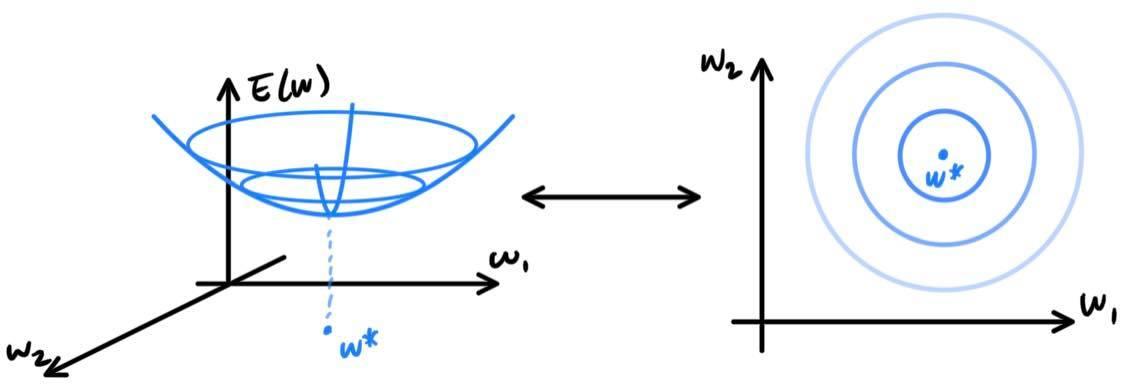
\includegraphics[width=0.6\textwidth]{img/ED(W).jpg}
    \caption{Error function contours in $\mathbb{R}^2$}
  \end{figure}

  To develop an intuition for this, let us visualize what this regularization term does. Setting $w \in \mathbb{R}^2$ for visual purposes, we can visualize the (unregularized) error function $E_D (w)$ as being defined over $\mathbb{R}^2$ with contours, where darker lines represent lower values. Clearly, the minimum value of $w$ lies at the dot $w^*$.

  \begin{figure}[H]
    \centering
    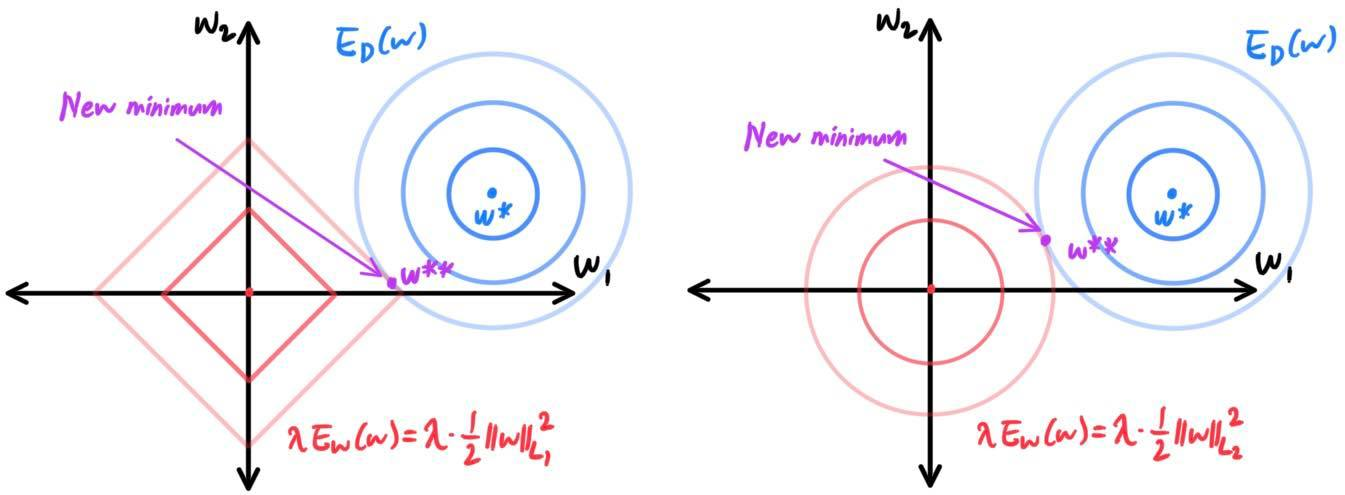
\includegraphics[width=0.9\textwidth]{img/L1vsL2.jpg}
    \caption{Comparison of L1 and L2 regularization effects}
  \end{figure}

  [Continuing with the rest of the visualizations and explanations...]

  In summary:
  \begin{itemize}
    \item The Laplace prior promotes sparsity, i.e. zeroes out some of the coefficients due to its greater peak around $0$.
    \item The Gaussian prior is more diffused around $0$, allowing non-zero values to have greater probability mass.
  \end{itemize}

  Other possibilities for robust priors are Cauchy or t-distributions.

\subsection{Bayesian Linear Regression with Gaussian Priors}

  To perform linear regression in the Bayesian setting, let us start off with a collection of potential models $\{\mathcal{M}_i\}_{i=1}^L$ and dataset $\mathcal{D}$. For each model $\mathcal{M}_i$ with
  \begin{equation}
    y = w^T \phi(x) + \epsilon, \;\;\;\;\; \epsilon \sim \mathcal{N}(0, \beta^{-1})
  \end{equation}

  We will state our unknowns:
  \begin{itemize}
    \item The value of $\beta$ that determines the variance of the error $\epsilon$ will have a \textit{fixed} prior distribution $p(\beta)$ (with no hyperparameter).
    \item The parameter $w$ has a (not fixed) prior distribution $p(w) = \mathcal{N}(w\,|\,0, \alpha^{-1} I)$ with hyperparameter $\alpha$.
    \item The value of $\alpha$ that determines the covariance matrix of the prior of $w$ will have a fixed prior distribution $p(\alpha)$, with no further hyperparameters.
  \end{itemize}

  Now, our final goal is to construct the predictive function $p(y\,|\,x, \mathcal{D})$. But since the predictive function is completely determinant on the values of $w, \beta$ (since $y = w^T \phi(x) + \epsilon \sim \mathcal{N}\big( w^T \phi(x), \beta^{-1}\big)$, we simply marginalize over the two parameters to simplify it into
  \begin{align*}
    p(y\,|\,x, \mathcal{D}) & = \iint p(y\,|\, x, w, \beta, \mathcal{D}) \, p(w, \beta \,|\,\mathcal{D})\; dw\, d\beta \\
    & = \iint \mathcal{N}\big(y\,|\, w^T \phi(x), \beta^{-1}\big) \, p(w, \beta\,|\, \mathcal{D})\; dw\, d\beta
  \end{align*}

  Therefore, we now need to calculate the joint posterior distribution of $w, \beta$ given $\mathcal{D}$. To marginalize this over the proper parameters, we need more insight.
  \begin{itemize}
    \item Let us first calculate $p(w\,|\,\mathcal{D})$ to see what parameters the posterior density is dependent on.
    \begin{align*}
      p(w\,|\,\mathcal{D}) & \propto p(\mathcal{D} \,|\,w)\, p(w) \\
      & = \Bigg( \int p(\mathcal{D}\,|\,w, \beta) \, p( \beta) \; d\beta \Bigg) \cdot \Bigg( \int p(w\,|\,\alpha)\, p(\alpha)\; d\alpha \Bigg) \\
      & = \int \bigg( \prod_{n=1}^N p(y_i\,|\,x_i, w, \beta)\bigg)\, p(\beta) \; d\beta \cdot \Bigg( \int \mathcal{N}(w\,|\,0, \alpha^{-1} I)\, p(\alpha)\; d\alpha \Bigg) \\
      & = \int \bigg( \prod_{n=1}^N \mathcal{N}\big( y\,|\, w^T \phi(x), \beta^{-1} \big) \bigg)\, p(\beta) \; d\beta \cdot \Bigg( \int \mathcal{N}(w\,|\,0, \alpha^{-1} I)\, p(\alpha)\; d\alpha \Bigg)
    \end{align*}
    
    Note that in this case, we marginalized over all $\beta$ and $\alpha$, so $p(w\,|\,\mathcal{D})$ is parameterized by both $\alpha$ and $\beta$. If we kept them fixed, we would have
    \begin{align*}
      p(w\,|\,\alpha, \beta, \mathcal{D}) & \propto p(\mathcal{D}\,|\,w, \alpha, \beta) \, p(w\,|\,\alpha, \beta) \\
      & = p(\mathcal{D}\,|\,w, \beta) \, p(w\,|\,\alpha) \\
      & = \bigg( \prod_{n=1}^N \mathcal{N}\big( y\,|\, w^T \phi(x), \beta^{-1} \big) \bigg) \cdot \mathcal{N}(w\,|\,0, \alpha^{-1} I) \\
      & = \mathcal{N}\big( w\,|\, m_N = \beta S_N \Phi^T \mathbf{Y}, S_N = (\alpha I + \beta \Phi^T \Phi)^{-1} \big)
    \end{align*}
    which itself is a multivariate Gaussian.
  \end{itemize}

  Knowing this, we know we should marginalize $p(w, \beta\,|\,\mathcal{D})$ so that the term $p(w\,|\, \alpha, \beta, \mathcal{D})$ exists. We can do this by
  \begin{align*}
    p(w, \beta\,|\,\mathcal{D}) & = \int p(w, \beta\,|\,\alpha, \mathcal{D}) \, p(\alpha\,|\,\mathcal{D})\; d\alpha \\
    & = \int p(w\,|\,\beta, \alpha, \mathcal{D}) \, p(\beta \,|\, \alpha, \mathcal{D}) \, p(\alpha\,|\,\mathcal{D}) \; d\alpha \\
    & = \int p(w\,|\, \beta, \alpha, \mathcal{D}) \, p(\alpha, \beta\,|\,\mathcal{D}) \; d\alpha
  \end{align*}

  where in the second row we simply used the conditional probability rule $p(a, b\,|\,c) = p(a\,|\,b, c)\, p(b\,|\,c)$. Finally, substituting this into the double integral above gives
  \begin{align*}
    p(y\,|\,x, \mathcal{D}) & = \iint p(y\,|\,x, w, \beta, \mathcal{D}) \, \bigg( \int p(w\,|\, \beta, \alpha, \mathcal{D}) \, p(\alpha, \beta\,|\,\mathcal{D}) \; d\alpha\bigg) \; dw\, d\beta \\
    & = \iiint p(y\,|\,x, w, \beta, \mathcal{D}) \, p(w\,|\, \beta, \alpha, \mathcal{D}) \, p(\alpha, \beta\,|\,\mathcal{D}) \; d\alpha \,dw\, d\beta \\
    & = \iiint \mathcal{N}\big(y\,|\, w^T \phi(x), \beta^{-1}\big)\,\bigg( \prod_{n=1}^N \mathcal{N}\big( y\,|\, w^T \phi(x), \beta^{-1} \big) \bigg) \cdot \mathcal{N}(w\,|\,0, \alpha^{-1} I)\, p(\alpha, \beta\,|\,\mathcal{D}) \; d\alpha \, dw \, d\beta
  \end{align*}



  Our Gaussian assumption on the priors will greatly simplify this term when written in vector notation. Now, the only thing to do is figure out what $p(\alpha, \beta\,|\,\mathcal{D})$ is. We will use Bayes rule and assume that the prior $p(\alpha, \beta)$ is relatively flat.
  \begin{align*}
    p(\alpha, \beta \,|\,\mathcal{D}) & \propto p( \mathcal{D}\,|\,\alpha, \beta) \, p(\alpha, \beta) \\
    & \propto p(\mathcal{D}\,|\,\alpha, \beta)
  \end{align*}

  where $p(\mathcal{D}\,|\,\alpha, \beta)$ is another evidence function (like the model evidence), which we will call the \textit{hyperparameter evidence}. We can simply condition over $w$ to get the following. Hopefully, the realizations of the probabilities into the densities function make sense to the reader.
  \begin{align*}
    p(\alpha, \beta \,|\, \mathcal{D}) & \propto p(\mathcal{D}\,|\,\alpha, \beta) \\
    & = \int p(\mathcal{D}\,|\,w, \beta) \, p(w \,|\,\alpha)\; dw \\
    & = \int \bigg(\prod_{n=1}^N \mathcal{N} \big(y_n \,|\, w^T \phi(x_n), \beta^{-1} \big)\bigg) \cdot \mathcal{N}(w\,|\, 0, \alpha^{-1} I)\; dw
  \end{align*}

  If we know that $p(\alpha, \beta \,|\,\mathcal{D})$ is sharply peaked, then we can try maximizing the evidence function with respect to $\alpha, \beta$ using maximum likelihood, and simply fixing them in further calculations.

  By substituting in the densities, the evidence function reduces to
  \begin{equation}
    p(\mathcal{D}\,|\,\alpha, \beta) = \bigg(\frac{\beta}{2 \pi}\bigg)^{N/2} \alpha^{M/2} \exp\big( -E (m_N)\big) \,|A|^{-1/2}
  \end{equation}
  where
  \begin{align*}
    \Phi & = (\Phi)_{nj} = \phi_j (x_n) \\
    S_N^{-1} & = \alpha I + \beta \Phi^T \Phi \\
    m_N & = \beta S_N \Phi^T \mathbf{Y} \\
    E(m_N) & = \frac{\beta}{2} ||\mathbf{Y} - \Phi m_N||^2 + \frac{\alpha}{2} m_N^T m_N
  \end{align*}

  Taking the log gives us
  \begin{equation}
    \log{p(\mathcal{D}\,|\,\alpha, \beta)} = \frac{M}{2}\log{\alpha} + \frac{N}{2} \log{\beta} - E(m_N) - \frac{1}{2} \log{|S_N^{-1}|} - \frac{N}{2} \log{2 \pi}
  \end{equation}

  This evidence can also be used as the model evidence. Remember that given data $\mathcal{D}$, a (linear) model $\mathcal{M}_i$ determines the collection of basis function, i.e. determines $\Phi$. Let us denote the $\Phi$ determined by model $\mathcal{M}_i$ as $\Phi_{\mathcal{M}_i}$. Therefore, we can treat $p(\mathcal{D}\,|\,\alpha, \beta)$ as a function of $\Phi$ and write
  \begin{equation}
    p(\mathcal{D}\,|\,\alpha, \beta, \Phi)
  \end{equation}

  To determine which model from $\{\mathcal{M}_i\}_{i=1}^L$ to choose, we first fix $\Phi_{\mathcal{M}_i}$ and maximize $p(\mathcal{D}\,|\,\alpha, \beta, \Phi_{\mathcal{M}_i})$ with respect to $\alpha, \beta$, for $i = 1, \ldots, L$.
  \begin{align*}
    \text{Assume model } \mathcal{M}_1 & \implies \text{Find } \max_{\alpha, \beta} p(\mathcal{D}\,|\,\alpha, \beta, \Phi_{\mathcal{M}_1}) \\
    \text{Assume model } \mathcal{M}_2 & \implies \text{Find } \max_{\alpha, \beta} p(\mathcal{D}\,|\,\alpha, \beta, \Phi_{\mathcal{M}_2}) \\
    \ldots & \implies \ldots \\
    \text{Assume model } \mathcal{M}_L & \implies \text{Find } \max_{\alpha, \beta} p(\mathcal{D}\,|\,\alpha, \beta, \Phi_{\mathcal{M}_L})
  \end{align*}

  Then, find
  \begin{equation}
    \text{arg}\, \max_{\mathcal{M}_i} \{ \max_{\alpha, \beta} p(\mathcal{D}\,|\,\alpha, \beta, \Phi_{\mathcal{M}_i}) \}
  \end{equation}

  For each model $\mathcal{M}_i$, we have optimized $\alpha, \beta$ to maximize the evidence function $p(\mathcal{D}\,|\,\alpha, \beta, \Phi_{\mathcal{M}_i})$. The model with the highest max evidence should be the best model, and by Occam's razor, we should choose simpler models if their predictive powers are equal. Again, we restate the big takeaway: \textit{The $\Phi$ represents the model, and therefore maximizing the evidence function $p(\mathcal{D}\,|\, \alpha, \beta, \Phi_{\mathcal{M}_i})$ with respect to the $\Phi$ will tell us what the correct model is.} That is,
  \begin{enumerate}
    \item $p(\mathcal{D}\,|\, \alpha, \beta, \Phi_{\mathcal{M}_i})$ interpreted as a function of $\alpha, \beta$ is the \textbf{hyperparameter evidence}.
    \item $p(\mathcal{D}\,|\, \alpha, \beta, \Phi_{\mathcal{M}_i})$ interpreted as a function of $\Phi_{\mathcal{M}_i}$ (or more accurately, of $\mathcal{M}_i$) is the \textbf{model evidence}.
  \end{enumerate}


